\documentclass[12pt]{report}

\title{Decentralised location proof system}

\usepackage[utf8]{inputenc}
\usepackage{graphicx}
\usepackage{subcaption}

\usepackage{tikz}
\usetikzlibrary{matrix,positioning,arrows.meta,arrows,calc}
\usepackage{enumitem}
\usepackage{float}
\usepackage{subfig}

\author{Conor Taylor}
\date{
	B.A.(Mod.) Computer Science\\
	Final Year Project, April 2016\\
	Supervisor: Stephen Barrett
}

\begin{document}
\maketitle

\tableofcontents
\newpage

\listoffigures
\newpage

\chapter{Introduction}
\section{Project and Motivation}
Location verification is the process of verifying whether a \textit{node} (computer) is physically present at a location it claims to be. Existing location proof systems attept to use centralised, trusted ``authoritive'' nodes to provide proof of another node's location. These approaches require investment in infrastructure, and are subject to privacy violation and denial of service attacks. This project aims to present a \textit{decentralised} solution to this problem. A decentralised location proof system is a system in which there is no ``authoritive source'' trusted and relied upon to provide and store sensitive location information.

This project describes a decentralised location proof system that is capable of operating on \textit{mobile nodes} (mobile devices). I propose a design in which location proofs are obtained using other untrusted mobile nodes as \textit{alibi's}. Proofs will be created as two mobile nodes communicate over an ad-hoc bluetooth network, transfer encrypted location information, and publish it on a public append-only bulletin board, known as a \textit{blockchain}. The decentralised nature of the system means that there is no single point of failure, no entity controlling the security of every node's location proofs, and no entity capable of violating another node's privacy. This is because in a decentralised system, no node is ``in charge'', and no node has more authority in the system than any other node.

\chapter{Background}
\section{Background}
\subsection{Proving your location}
As an increasing amount of personal information is accessible on the internet and therefore on mobile devices, the security that existed by requiring physical interaction between humans to transfer sensitive data is lost.

\subsection{Ad-hoc networks}

\subsection{Blockchain}

\subsection{Centralised location proof systems}
Location proof systems are expected to be accurate and tamper-proof. For this reason, existing solutions have chosen to use a central authority to issue proofs, or to regulate proof issuance \cite{brassil, luo, khan}.

A hardware technique \cite{brassil} operates by supplementing existing WiFi access points with \textit{femtocells}. A femtocell is a small cellular antenna that connects to a mobile carrier via the Internet. Location verification over the internet is made possible by determining which femtocell a mobile node is connected to as it transfers data via Wi-Fi. This solution requires investment in additional hardware to supplement existing WiFi access points, and requires access to mobile providers' user database to identify users locations.

The use of a centralised system, like that described by Brassil et al. \cite{brassil}, creates security, privacy and vulnerability issues. An attacker who succeeds in compromising the security of the central server can violate the privacy of the users of the system, and potentially track their location. The central system architecture is also vulnerable, in the sense that a resource availability attack such as a DDoS attack could render the central architecture unavailable, making location verification unavailable.

Luo et al. propose a system that uses Wi-Fi access points (\textit{AP's}) to allow users to create location proofs \cite{luo}. In their system, each access point has a \textit{group signature} and can sign location proofs for requesting users. Users can request a location proof from any access point, and receive a proof encrypted by the AP with the group signature, as shown in figure \ref{fig:luo_transaction}. This can then be submitted to a Verifier.

\begin{figure}[H]
\begin{center}
\resizebox {0.6\columnwidth} {!} {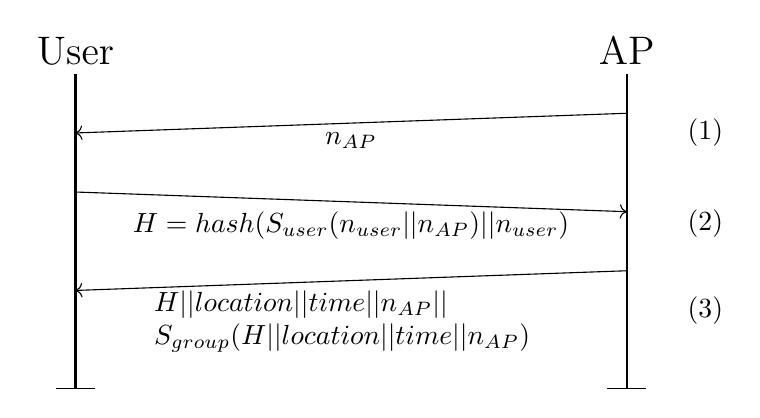
\begin{tikzpicture}
\coordinate (A_T) at (0,3);
\coordinate (A_B) at (0,-1);
\coordinate (A_1) at (0,2.25);
\coordinate (A_2) at (0,1.5);
\coordinate (A_3) at (0,0.25);
\coordinate (A_BL) at (-0.25,-1);
\coordinate (A_BR) at (0.25,-1);

\coordinate (B_T) at (7,3);
\coordinate (B_B) at (7,-1);
\coordinate (B_1) at (7,2.5);
\coordinate (B_2) at (7,1.25);
\coordinate (B_3) at (7,0.5);
\coordinate (B_BL) at (6.75,-1);
\coordinate (B_BR) at (7.25,-1);

\draw[-] (A_BL) -- (A_BR);
\draw[-] (B_BL) -- (B_BR);

\coordinate (L_1) at (8,2.25);
\coordinate (L_2) at (8,1.1);
\coordinate (L_3) at (8,0);

\node at (L_1) {(1)};
\node at (L_2) {(2)};
\node at (L_3) {(3)};

\draw[thick] (A_T)--(A_B);
\draw[thick] (B_T)--(B_B);
\draw (A_T) node[above]{\Large User};
\draw (B_T) node[above]{\Large AP};

\draw[->] (B_1) -- (A_1) node[midway,below] {$n_{AP}$};
\draw[->] (A_2) -- (B_2) node[midway,below]
	{$H = hash(S_{user}(n_{user} || n_{AP}) || n_{user})$};
	
\draw[->] (B_3) -- (A_3) node[text width=5cm,midway,below]
	{$H || location || time || n_{AP} ||$\\
	$S_{group}(H || location || time || n_{AP})$};
\end{tikzpicture}}
\end{center}
\caption{Adopted from Luo et al. \cite{luo}}
\label{fig:luo_transaction}
\end{figure}

This kind of system creates \textit{proactive} location proofs. A proactive location proof is one which is created before it is needed. The user creates application-independent location proofs, and can use them at a later time with any application(s) he chooses.

\chapter{Design}
\section{Design}
The location proof system we propose allows \textit{mobile nodes} to create location proofs for each other after physically meeting. When two mobile nodes are in close physical proximity, they initiate a transaction over a short range, ad-hoc network such as Bluetooth.

To create a transaction, two mobile nodes anonymously share their GPS coordinates and current time over a short-range network. Both nodes then check that these parameters don't differ by more than some value $\epsilon$. Once satisfied, they each create an encrypted, privacy-protecting transaction logging their location and the identity of the other mobile node (the \textit{alibi}) used to create the transaction. This transaction is published onto a public, append-only bulletin board known as a \textit{blockchain} \cite{blueprint}.

Once given permission from a mobile node (by transferring decryption keys), a \textit{Verifier node} can consult the data in blockchain and determine whether or not the mobile node is present at its claimed location. The blockchain is managed by a network of \textit{Miner nodes}, who collect transactions from mobile nodes, distribute them across the network, and try to create a new \textit{block} of transactions by attempting to solve a \textit{proof-of-work} puzzle.

Any mobile node acting as an alibi in a transaction will share details of its most recent transactions with the other mobile node in the transaction. This means that when the mobile node seeks verification from a Verifier node, the Verifier can examine the mobile node's alibi's, and each of the alibi's recent alibi's, forming a large graph of connections which can be used to verify or reject the mobile nodes claimed location. Only the owner of the transaction can give permission to a Verifier to check its location history, by providing the Verifier with the keys needed to decrypt the transactions.

Figure \ref{fig:overview} provides an overview of the operation of the proposed system.

\begin{figure}[H]
\begin{center}
\resizebox {\columnwidth} {!} {\includegraphics{diagrams/overview.png}}
\caption{Design and operation overview}
\label{fig:overview}
\end{center}
\end{figure}

\begin{enumerate}[label=\textbf{\arabic*}.]
\item Two mobile nodes in close physical proximity create a transaction.
\item The mobile nodes each publish their transaction to a Miner node.
\item The Miner node distributes the transaction across the Miner network.
\item One Miner node solves the proof-of-work for a block of transactions, and the new block of transactions is appended to the blockchain.
\item A mobile node requests verification from a Verifier node (request structure is explained in section \ref{ssec:verification}).
\item The Verifier node uses the public blockchain to examine the requesting node's transactions and determine their validity.
\item The Verifier accepts or rejects the  mobile node's claimed location based on its transactions in the blockchain. 
\end{enumerate}

\subsection{Identities}
In order to preserve user's privacy, a user will only ever use an identity for one transaction, before generating a new one. This prevents curious users from watching the public blockchain for a known identity and tracking it. However, to prevent identity theft, it is important for the Verifier to be able to prove that a mobile node is the owner of each identity. This is achieved using a public/private key pair for each mobile node.

When a mobile node is created, it generates a public/private key pair. To maintain anonymity, the mobile node will use the public key to encrypt \textit{nonces} to create \textit{identities}, and use these to identify itself in a transaction. A different identity will be created for each transaction. During the verification stage, the node will provide the Verifier with its public key, along with the list of the nonces used to generate its $n$ most recent transactions (see figure \ref{fig:verify_request}). This allows the Verifier to calculate all of the node's identities, and prove that they were all created by the same node, and can then retrieve the transactions associated with those identities from the blockchain. The Verifier will also ensure that the node owns the private key associated with the provided public key, to prevent identity theft.

\subsubsection{Nonce list} \label{sssec:nonce_list}
A \textit{Nonce List} is simply a list of all of the nonces a mobile node has used so far to generate identities. When a mobile node generates a new identity, it must first generate a new nonce which is then encrypted to create the identity. The nonce is appended to the mobile node's nonce list, so it can be used later during verification (see section \ref{ssec:verification}).

\subsubsection{Identity duplication}
Since all identities are generated from random nonces, there is nothing to stop two nodes from generating the same identity and using it in different transactions. It is therefore possible that during verification, a Verifier node may find multiple transactions with the same ID in the blockchain. The Verifier will have a decryption key for the transaction it is searching for, which will only be able to decrypt one of the transactions with the duplicate ID. The Verifier will try to decrypt each one until it finds one that can be decrypted successfully.

\newpage
\subsection{Transactions} \label{sec:transactions}
During a transaction between two nodes, a number of different items must be shared and calculated. Figure \ref{fig:transaction} describes an honest, successful transaction, assuming an ad-hoc Bluetooth network has already been set up between nodes $A$ and $B$.

\begin{figure}[H]
\resizebox {\columnwidth} {!} {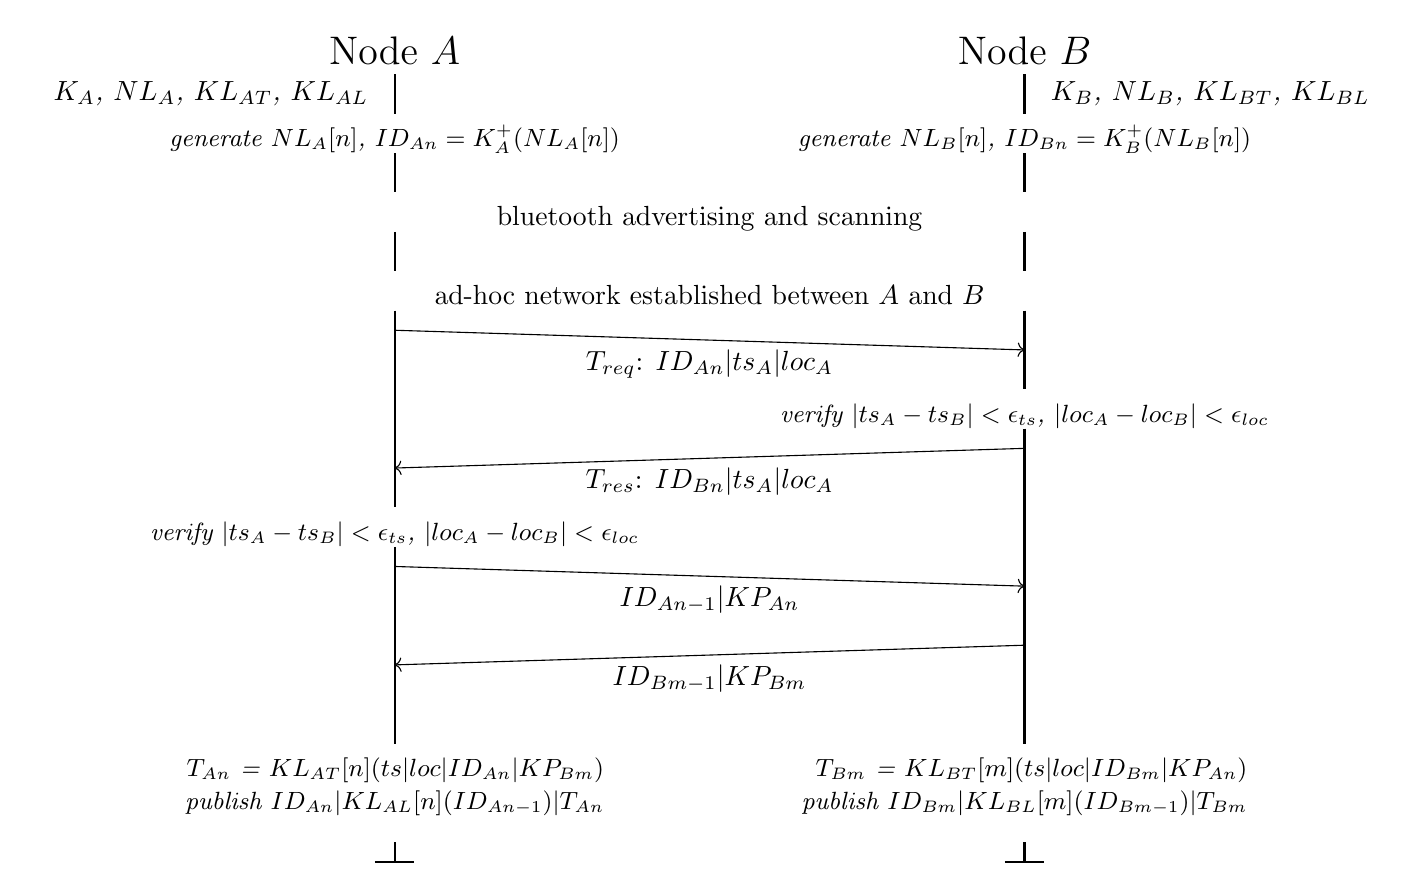
\begin{tikzpicture}
\coordinate (A_1) at (0,10);
\coordinate (A_2) at (0,9.5);
\coordinate (A_3) at (0,9);
\coordinate (A_4) at (0,8.5);
\coordinate (A_5) at (0,8);
\coordinate (A_6) at (0,7.5);
\coordinate (A_7) at (0,7);
\coordinate (A_8) at (0,4.5);
\coordinate (A_9) at (0,4);
\coordinate (A_10) at (0,1.5);
\coordinate (A_11) at (0,0.25);
\coordinate (A_12) at (0,0);
\coordinate (AF_L) at (-0.25,0);
\coordinate (AF_R) at (0.25,0);

\coordinate (M_1) at (4,8.5);
\coordinate (M_2) at (4,7.5);

\coordinate (B_1) at (8,10);
\coordinate (B_2) at (8,9.5);
\coordinate (B_3) at (8,9);
\coordinate (B_4) at (8,8.5);
\coordinate (B_5) at (8,8);
\coordinate (B_6) at (8,7.5);
\coordinate (B_7) at (8,7);
\coordinate (B_8) at (8,6);
\coordinate (B_9) at (8,5.5);
\coordinate (B_10) at (8,1.5);
\coordinate (B_11) at (8,0.25);
\coordinate (B_12) at (8,0);
\coordinate (BF_L) at (7.75,0);
\coordinate (BF_R) at (8.25,0);

\draw[thick] (A_1)--(A_2) (A_3)--(A_4) (A_5)--(A_6) (A_7)--(A_8) (A_9)--(A_10) (A_11)--(A_12) (AF_L)--(AF_R);
\draw[thick] (B_1)--(B_2) (B_3)--(B_4) (B_5)--(B_6) (B_7)--(B_8) (B_9)--(B_10) (B_11)--(B_12) (BF_L)--(BF_R);
\draw (A_1) node[above]{\Large Node $A$};
\draw (B_1) node[above]{\Large Node $B$};

\draw ($(A_1)!.5!(A_2)$) node[left]{\begin{tabular}{r}
\textit{$K_A$, $NL_A$, $KL_{AT}$, $KL_{AL}$}
\end{tabular}};

\draw ($(B_1)!.5!(B_2)$) node[right]{\begin{tabular}{r}
\textit{$K_B$, $NL_B$, $KL_{BT}$, $KL_{BL}$}
\end{tabular}};

\draw (A_2) node[below,text centered]{\begin{tabular}{r}
\small{\textit{generate $NL_A[n]$, $ID_{An} = K^{+}_A(NL_A[n])$}}
\end{tabular}};

\draw (B_2) node[below,text centered]{\begin{tabular}{r}
\small{\textit{generate $NL_B[n]$, $ID_{Bn} = K^{+}_B(NL_B[n])$}}
\end{tabular}};

\draw (M_1) node[below,text centered]{\begin{tabular}{r}
bluetooth advertising and scanning
\end{tabular}};

\draw (M_2) node[below,text centered]{\begin{tabular}{r}
ad-hoc network established between $A$ and $B$
\end{tabular}};

\coordinate (AX_1) at ($(A_7)-(0,0.25)$);
\coordinate (BX_1) at ($(B_7)-(0,0.5)$);
\draw[->] (AX_1) -- (BX_1) node[midway,below]
	{$T_{req}$: $ID_{An} | ts_A | loc_A$};
	
\draw (B_8) node[below,text centered]{\begin{tabular}{r}
\small{\textit{verify $|ts_A-ts_B| < \epsilon_{ts}$, $|loc_A-loc_B| < \epsilon_{loc}$}}
\end{tabular}};

\coordinate (AX_2) at ($(A_7)-(0,2)$);
\coordinate (BX_2) at ($(B_9)-(0,0.25)$);
\draw[->] (BX_2) -- (AX_2) node[midway,below]
	{$T_{res}$: $ID_{Bn} | ts_A | loc_A$};
	
\draw (A_8) node[below,text centered]{\begin{tabular}{r}
\small{\textit{verify $|ts_A-ts_B| < \epsilon_{ts}$, $|loc_A-loc_B| < \epsilon_{loc}$}}
\end{tabular}};

\coordinate (AX_3) at ($(A_9)-(0,0.25)$);
\coordinate (BX_3) at ($(B_9)-(0,2)$);
\draw[->] (AX_3) -- (BX_3) node[midway,below]
	{$ID_{An-1}|KP_{An}$};

\coordinate (AX_4) at ($(A_9)-(0,1.5)$);
\coordinate (BX_4) at ($(B_9)-(0,2.75)$);
\draw[->] (BX_4) -- (AX_4) node[midway,below]
	{$ID_{Bm-1}|KP_{Bm}$};

\draw (A_10) node[below,text centered]{\begin{tabular}{r}
\small{\textit{$T_{An}$ = $KL_{AT}[n](ts|loc|ID_{An}|KP_{Bm})$}}\\
\small{\textit{publish $ID_{An}|KL_{AL}[n](ID_{An-1})|T_{An}$}}
\end{tabular}};

\draw (B_10) node[below,text centered]{\begin{tabular}{r}
\small{\textit{$T_{Bm}$ = $KL_{BT}[m](ts|loc|ID_{Bm}|KP_{An})$}}\\
\small{\textit{publish $ID_{Bm}|KL_{BL}[m](ID_{Bm-1})|T_{Bm}$}}
\end{tabular}};
\end{tikzpicture}}
\caption{Honest, successful transaction}
\label{fig:transaction}
\end{figure}

Where:
\begin{itemize}[noitemsep,topsep=0pt]
	\item[] $\mathbf{NL_A[n]}$ is the $n$th nonce in $A$'s \textit{Nonce List}, which is used to generate $ID_{An}$ (see section \ref{sssec:nonce_list}).
\end{itemize}

\null
When a node is initialised, it must begin to record two \textit{Key Lists} for itself. A \textit{Key List} is a list of encryption keys previously used for transactions. For example, $KL_{AT}[n]$ and $KL_{AL}[n]$ are the two keys used to encrypt node $A$'s $n$th transaction and matching chronological link, respectively. These \textit{Key Lists} and are assumed to have been initialised and populated before the transaction described in Figure \ref{fig:transaction} begins.

After creating an ad-hoc Bluetooth network between nodes $A$ and $B$, the first step in the transaction is for both nodes to share their IDs, and agree upon a GPS location and current time. Nodes likely won't share the exact same GPS coordinates or time, but once the values don't differ by more than some small constant $\epsilon$, the nodes will continue with the transaction. If node $A$ claims a GPS location or timestamp that differs from what node $B$ senses by more than $\epsilon$, node $B$ will abort the transaction.

After nodes agree upon the parameters of the transaction, they exchange their previous ID, along with their \textit{Key Packets}. A \textit{Key Packet} is a list of keys used in a node's $n$ most recent transactions, along with the transaction ID's if necessary. This allows node $A$ to decrypt node $B$'s $m$ most recent transactions, therefore providing an alibi for node $A$.

\subsubsection{Transaction creation}
Once nodes have exchanged \textit{Key Packets}, their communication is finished and they can close their ad-hoc channel. Each node creates a new transaction object, $T$, to publish onto the public blockchain. The following transaction data will be calculated by node $A$, after communicating with node $B$:
\\

$T_{An} = KL_{AT}[n](ts|loc|ID_{An}|KP_{Bm})$
\\

Where:
\begin{itemize}[noitemsep,topsep=0pt]
	\item[] $\mathbf{n}$ is node $A$'s current transaction number (i.e. $A$ has published $n-1$ transactions before now).
	\item[] $\mathbf{KL_{AT}}$ is one of $A$'s \textit{Key Lists}, used to encrypt transactions.	
	\item[] $\mathbf{ts}$ is the timestamp of the transaction, as recorded by node $A$.
	\item[] $\mathbf{loc}$ is the GPS coordinates of the transaction, as recorded by node $A$.
	\item[] $\mathbf{ID_{An}}$ is $A$'s $nth$ identity, used for this transaction only.
	\item[] $\mathbf{KP_{Bm}}$ is $B$'s \textit{Key Packet} at time $m$. Its exact contents are discussed in more detail in section \ref{sssec:key_packets}
\end{itemize}

\subsubsection{Publishing to the blockchain}
After creating $T_{An}$, node $A$ must publish it to the public blockchain. The data published must be searchable in order to provide a Verifier with some way of identifying specific transactions. Nodes use their current ID as the identifier for the transaction.

\textit{Backwards-chaining} is an important part of verifiability. The Verifier must be able to prove that the proof chain provided by the mobile node has not been chronologically re-ordered. The transaction must therefore be accompanied by a link to the node's chronologically previous transaction. This link must be encrypted, along with the transaction timestamp, to prevent a curious user from monitoring the public blockchain to observe a user's transaction publishing activity. $A$'s copy of the transaction log $P_{An}$ will therefore be in the form:
\\

$P_{An} = ID_{An}|KL_{AL}[n](ID_{An-1}|ts_A)|T_{An}$

\null
To publish $P_{An}$, $A$ must send $P_{An}$ to a miner node, who will add it to its \textit{pending transaction} queue, and send it to other miners in the network to add it to their queues as well. The transaction will then be signed into the next block in the blockchain.

\subsubsection{Key Packets} \label{sssec:key_packets}
The key packet is more than simply a list of keys that a mobile node has used to encrypt its transactions; in order to preserve the ``selective in-sequence privacy'' property of OTIT \cite{otit}, a user must be able to choose transactions that he doesn't want others to be able to decrypt. However, in order to simultaneously preserve OTIT's ``privacy protected chronology'' property, the transaction backwards-chaining must not be broken. This is why two separate \textit{Key Lists} are maintained; $KL_{AL}$ is used to encrypt the backwards-chaining link and transaction timestamp, while $KL_{AT}$ encrypts the transaction data. For example, if node $B$ doesn't want to reveal transaction $T_{Bm-1}$, he would reveal the following key packet:
\\

${KP_{Bm} = (\{KL_{BL}[m], KL_{BT}[m]\}, KL_{BL}[m-1], \{KL_{BL}[m-2], KL_{BT}[m-2]\})}$

\null
In this case, $KL_{BT}[m-1]$ has not been included with $KL_{BL}[m-1]$, in order to protect the privacy of this transaction. This may be needed, for example, if node $B$ doesn't want to allow anyone to decrypt any transactions he has created withing 5km of his home, in order to protect his privacy.

\subsubsection{Aborting transactions}
A node may decide to abort a transaction if it thinks it is in contact with a malicious node. In figure \ref{fig:aborted_transaction}, node $A$ encounters a malicious node $M$, who tries to spoof its identity with $A$. Node $A$ will abort the transaction once it notices that $|ts_A-ts_M| \geq \epsilon_{ts}$, or $|loc_A-loc_M| \geq \epsilon_{loc}$.

To abort the transaction, $A$ terminates the ad-hoc network with node $M$, and won't publish anything onto the blockchain. This means that even if $M$ fabricates some data from $A$ and publishes a transaction onto the blockchain, the matching transaction from $A$ will not be present. Any transaction on the blockchain that do not contain a reference to a valid  alibi transaction will be disregarded during verification.

\begin{figure}[h]
\resizebox {\columnwidth} {!} {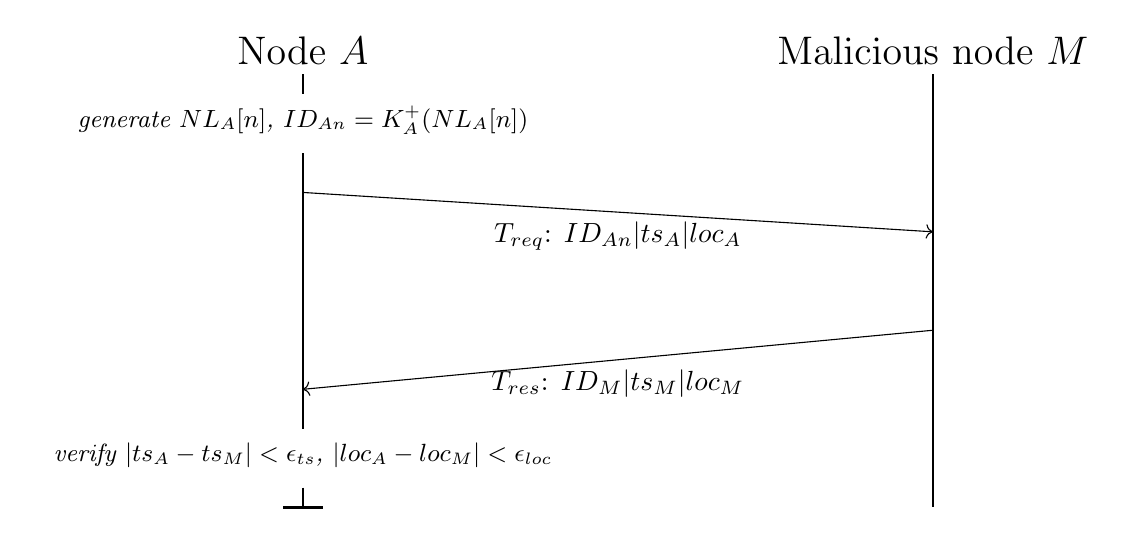
\begin{tikzpicture}
\coordinate (A_1) at (0,5.5);
\coordinate (A_2) at (0,5.25);
\coordinate (A_3) at (0,4.5);
\coordinate (A_8) at (0,1);
\coordinate (A_9) at (0,0.25);
\coordinate (A_12) at (0,0);
\coordinate (AF_L) at (-0.25,0);
\coordinate (AF_R) at (0.25,0);

\coordinate (B_1) at (8,5.5);
\coordinate (B_3) at (8,4.5);
\coordinate (B_8) at (8,3.25);
\coordinate (B_9) at (8,2.5);
\coordinate (B_12) at (8,0);

\draw[thick] (A_1)--(A_2) (A_3)--(A_8) (A_9)--(A_12) (AF_L)--(AF_R);
\draw[thick] (B_1)--(B_3) (B_3)--(B_9) (B_9)--(B_12);
\draw (A_1) node[above]{\Large Node $A$};
\draw (B_1) node[above]{\Large Malicious node $M$};

\draw (A_2) node[below,text centered]{\begin{tabular}{r}
\small{\textit{generate $NL_A[n]$, $ID_{An} = K^{+}_A(NL_A[n])$}}
\end{tabular}};

\coordinate (AX_1) at ($(A_3)-(0,0.5)$);
\coordinate (BX_1) at ($(B_3)-(0,1)$);
\draw[->] (AX_1) -- (BX_1) node[midway,below]
	{$T_{req}$: $ID_{An} | ts_A | loc_A$};

\coordinate (AX_2) at ($(A_3)-(0,3)$);
\coordinate (BX_2) at ($(B_8)-(0,1)$);
\draw[->] (BX_2) -- (AX_2) node[midway,below]
	{$T_{res}$: $ID_{M} | ts_M | loc_M$};
	
\draw (A_8) node[below,text centered]{\begin{tabular}{r}
\small{\textit{verify $|ts_A-ts_M| < \epsilon_{ts}$, $|loc_A-loc_M| < \epsilon_{loc}$}}
\end{tabular}};
\end{tikzpicture}}
\caption{An aborted transaction due to malicious node $M$}
\label{fig:aborted_transaction}
\end{figure}

\subsection{Verification} \label{ssec:verification}
\begin{minipage}{0.5\linewidth}
In the verification stage, a mobile node tries to prove its location to a Verifier node, e.g. a bank. To do this, the mobile node sends the Verifier a number of parameters, as shown in Figure \ref{fig:verify_request}:
\begin{itemize}[noitemsep,topsep=0pt]
	\item[] $\mathbf{ID_{An-1}}$ is the ID of $A$'s most recently published transaction.
	\item[] $\mathbf{KP_{An-1}}$ is $A$'s key packet up to transaction $n-1$, and includes keys for as many transactions as $A$ feels is appropriate in order to receive verification.
	\item[] $\mathbf{loc}$ is $A$'s current claimed GPS coordinates for which it is seeking verification.
	\item[] $\mathbf{NP_{An-1}}$ is $A$'s \textit{Nonce Packet}, a subset of its \textit{Nonce List} (section \ref{sssec:nonce_list}). A Nonce Packet is the list of the nonces used to generate $A$'s most recent IDs, up to $n-1$., that $A$ is willing to share with the Verifier. 
\end{itemize}
\end{minipage}
\hfill
\begin{minipage}[c]{0.5\linewidth}
\begin{figure}[H]
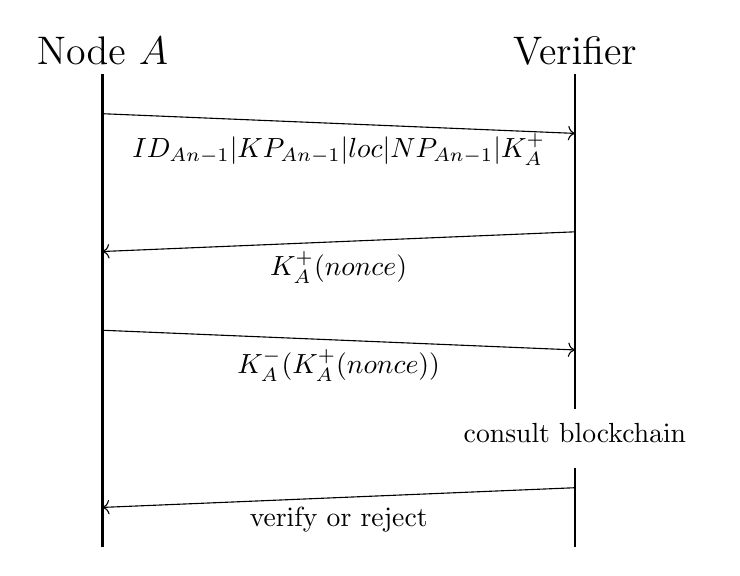
\begin{tikzpicture}
\coordinate (A_1) at (0,6);
\coordinate (A_2) at (0,0);

\coordinate (B_1) at (6,6);
\coordinate (B_2) at (6,1.75);
\coordinate (B_3) at (6,1);
\coordinate (B_4) at (6,0);

\draw[thick] (A_1)--(A_2);
\draw[thick] (B_1)--(B_2) (B_3)--(B_4);
\draw (A_1) node[above]{\Large Node $A$};
\draw (B_1) node[above]{\Large Verifier};

\coordinate (AX_1) at ($(A_1)-(0,0.5)$);
\coordinate (BX_1) at ($(B_1)-(0,0.75)$);
\draw[->] (AX_1) -- (BX_1) node[midway,below]
	{$ID_{An-1}|KP_{An-1}|loc|NP_{An-1}|K^{+}_A$};
	
\coordinate (AX_2) at ($(A_1)-(0,2.25)$);
\coordinate (BX_2) at ($(B_1)-(0,2)$);
\draw[->] (BX_2) -- (AX_2) node[midway,below]
	{$K^{+}_A(nonce)$};

\coordinate (AX_3) at ($(A_1)-(0,3.25)$);
\coordinate (BX_3) at ($(B_1)-(0,3.5)$);
\draw[->] (AX_3) -- (BX_3) node[midway,below]
	{$K^{-}_A(K^{+}_A(nonce))$};
	
\draw (B_2) node[below,text centered]{\begin{tabular}{r}
consult blockchain
\end{tabular}};

\coordinate (AX_2) at ($(A_1)-(0,5.5)$);
\coordinate (BX_2) at ($(B_1)-(0,5.25)$);
\draw[->] (BX_2) -- (AX_2) node[midway,below]
	{verify or reject};

\end{tikzpicture}
\caption{Verification request}
\label{fig:verify_request}
\end{figure}
\end{minipage}

The goal of the verification stage is for the Verifier to either accept or reject the location that the user is claiming. Given $ID_{An-1}$ and $KP_{An-1}$, a Verifier is able to retrieve $A$'s previous transactions, and the transactions of all of its alibi's.

The Verifier uses $NP_{An-1}$ and $K^{+}_A$ to prove that node $A$ was the author of all of the transactions he claims to be. This prevents a collusion attack whereby nodes could share common transactions between different proof chains. When walking chronologically backwards along $A$'s proof chain, the 3rd party will ensure that the ID used in transaction $m$ on the proof chain matches $K^{+}_A(NP_{An-1}[m])$.

There are a huge number of possible factors involved in reaching a conclusion from the data on the blockchain; some of these factors will likely be unique to certain Verifiers, and kept secret to improve reliability and avoid gaming. Some simple example factors may include:
\begin{itemize}
	\item \textbf{Alibi credibility:} if each of the node’s alibi’s have little or no alibi’s themselves, then the node is likely attempting a poorly-constructed Sybil attack, and the Verifier will reject his verification request.
	\item \textbf{Alibi reuse:} if the Verifier can prove that alibi’s are being reused frequently, then it will reject the verification request.
	\begin{itemize}
		\item Due to transaction anonymity, the Verifier may not always be able to tell if two alibi's are the same person or not. e.g. node $A$ could use node $B$ as an alibi, then wait for $B$ to complete $n$ more transactions, then use node $B$ again.
		\item This is not a viable attack on the verification system. Depending on the size of $n$, enough time may pass between both uses of node $B$ as an alibi that the transactions are no longer relevant.
	\end{itemize}
\end{itemize}

\chapter{Evaluation}
\section{Evaluation}
In this paper, we have presented a model for a location proof system which aims to preserve privacy and prevent false proofs from being created.

\subsection{OTIT conformance}
We can compare our model to OTIT \cite{otit}, a list of features and requirements necessary for designing any secure location proof scheme. OTIT presents 8 such requirements:
\begin{enumerate}
\item[] \textbf{Chronological}: The chronological property of OTIT ensures that transactions are published in the order they were created. In our system we do not enforce this property at the time of transaction publication. This is to avoid revealing any transaction information to the miner nodes, therefore preserving the privacy of the transaction owner. Instead, we enforce this property at the time of verification. The chronological link created by adding $KL_{AT}(ID_{A-1}|ts_A)$ to the transaction will allow Verifier nodes to prove that the transaction is chronologically ordered, preserving OTIT's ``Chronological'' property.

\item[] \textbf{Order preserving}: This property states that the order of transactions cannot be modified after they are created. In our system, a blockchain is used to store transactions. In a blockchain, new blocks are added in a linear, chronological order, and cannot be modified so long as the majority of miners in the network are honest \cite{blueprint}. Therefore the transactions stored in these blocks satisfy the ``Order preserving'' property of OTIT. % in the dissertation i can discuss ordering within a block here (and go into detail about the merkle root etc)

\item[] \textbf{Verifiable}: This states that the proof, and the order or proofs, should be verifiable by a trusted auditor. In our case, a Verifier node is an auditor trusted by the mobile node seeking verification. A Verifier node may be operated by a bank, government, or any entity wishing to make use of our location proof system.

Our system inherently satisfies this property of OTIT, as Verifier nodes are required to verify or reject a mobile node's claimed location. This is done by examining the mobile node's chronological link of transactions, and recursing for each alibi used for each transaction along the chronological link until the Verifier can conclude if the transaction chain is valid or not.

\item[] \textbf{Tamper evident}: Our system is tamper evident. If a malicious node creates a successful transaction with an honest node, but modifies the transaction data before publishing, a Verifier node will reject the malicious transaction. This rejection will be on the grounds that the matching transaction, published by the honest node, contains contradictory data.

We assume the underlying security of the blockchain, so any malicious miner nodes will not be able to tamper with existing transaction data providing that the majority of CPU power in the mining system is owned by honest miners \cite{bitcoin}. Therefore the tamper evident property is satisfied.

\item[] \textbf{Privacy preserved}: This states that the user should have control over his level of privacy exposure when using the system. In our system, this is provided using \textit{Key Lists} \ref{sec:transactions}. We provide two keys for each transaction; $KL_{AT}[n]$ is used to encrypt the \textit{transaction data} for $A$'s $nth$ transaction, and $KL_{AL}[n]$ is used to encrypt the \textit{backwards chronological link} between $A$'s $nth$ transaction and transaction $n-1$.

To control his privacy, a user can choose only to reveal $KL_{AL}[n]$ for a specific transaction $n$. This may be useful if a user does not wish to reveal transaction data for transactions created within a certain distance of his house, for example. Hiding $KL_{AT}[n]$ while revealing $KL_{AL}[n]$ has the advantage of preserving the user's privacy while maintaining a clear backwards chronological link of transactions for the Verifier to follow, preserving both privacy and system consistency.

\item[] \textbf{Selective in-sequence privacy}: This is the requirement that any proof chain must support \textit{sub-set verification}, allowing a user to provide only a sub-set of proofs from his current proof chain for verification. Our system satisfies this property by using \textit{Key Packets} (section \ref{sssec:key_packets}).

In our system, a \textit{sub-set} of $A$'s proof chain can be defined as $KP_{An}$. The sub-set therefore begins with $ID_{An}$, and ends when there is no key $KL_{AL}[n-m]$ in $KP_{An}$ to decrypt the link to transaction $T_{An-m-1}$. 

\item[] \textbf{Privacy protected chronology}: This states that the proof system, which provides \textit{selective in-sequence privacy}, should also ensure that the user does not ``hide away'' important items within the subset. This is impossible in our system due to the use of backwards chronological linking between transactions, so our model satisfies this property.

\item[] \textbf{Convenience and derivability}: This requirement states that the verification process should be convenient, and the user should not burden the Verifier node with a huge load of data. In our system, the data is stored in a central blockchain that the Verifier has access to, and the user provides the Verifier only with decryption keys and indexes into a sub-section of this data. Therefore the data sent to from the user to the Verifier, $KP_{An}$, is quite small in size.

The Verifier has the freedom to decide how comprehensively to investigate the user's data; It can bound how deeply to investigate the graph of alibi's, if at all. We therefore satisfy this requirement by allowing the Verifier to choose how complex the verification process needs to be.
\end{enumerate}

\subsection{Attacks on the system}
\subsubsection{Identity replication}
By repeatedly publishing fake transactions with the same ID, a malicious user can impede the Verification of certain transactions. This is because a Verifier will have to attempt to decrypt all transactions with the same ID until it finds one that decrypts successfully. A malicious user can therefore slow down the verification stage of certain transactions by flooding the blockchain with transactions with the same ID.

This is an abuse of the system than an attack. A malicious user will not be able to target specific users' transactions, because they are privacy protected. The malicious user can therefore gain no material advantage or compromise the security of the system by using an attack like this.

To avoid this attack, Miner nodes may reject any transactions with duplicate transaction IDs. Assuming sufficiently large transaction IDs, a duplicate ID is unlikely to happen through honest operation. Miners can assume that any transactions with duplicate IDs are malicious, and reject them.

\subsubsection{Sybil attack}
This system is vulnerable to a Sybil attack, where a single physical node may create multiple \textit{pseudoidentities} \cite{sybil}. A suitably powerful node, or motivated attacker, could create enough pseudonyms to create a subnetwork of nodes, each creating malicious transactions with each other. This would allow an attacker to falsify a believable location proof.

It has been proven that a central certificate authority is the only method of preventing a Sybil attack \cite{sybil}. Other measures, such as web of trust, increase the difficulty involved in performing an attack, but the system remains vulnerable to a motivated attacker.

\chapter{Future work}

\newpage
\begin{thebibliography}{9}

\bibitem{brassil}
  J. Brassil, P.K. Manadhata,
  ``Verifying the Location of a Mobile Device User'',
  Proc. of MobiSec 2012,
  June 2012.

\bibitem{luo}
  W. Luo, U. Hengartner,
  ``Proving your Location without giving up your Privacy'',
  Proceedings of the Eleventh Workshop on Mobile Computing Systems \& Applications,
  HotMobile 2010, Annapolis, Maryland, February 22 - 23, pp. 7–12. ACM,
  New York (2010).

\bibitem{khan}
  R. Khan, S. Zawoad, M. Haque, and R. Hasan,
  ```Who, When, and Where?' Location Proof Assertion for Mobile Devices'',
  Proceedings of the 28th Annual IFIP WG 11.3 Working Conference on Data and Applications Security and Privacy, ser. DBSec. IFIP,
  July 2014.
 
\bibitem{otit}
  R. Khan, S. Zawoad, M. Haque, and R, Hasan.
  ``OTIT: Towards secure provenance modeling for location proofs'',
  Proc. of ASIACCS. ACM (2014).

\bibitem{sybil}
  J.R. Douceur,
  ``The sybil attack'',
  Druschel, P., Kaashoek, M.F., Rowstron, A. (eds.) IPTPS 2002. LNCS, vol. 2429, pp. 251–260,
  Springer, Heidelberg (2002).

\bibitem{maxmind}
  MaxMind LLC. GeoIP. http://www.maxmind.com,
  2010.

\bibitem{constraint-based}
  B. Gueye, A. Ziviani, M. Crovella, and S. Fdida,
  ``Constraint-based geolocation of Internet hosts'',
  IEEE/ACM Transactions on Networking,
  14(6):1219–1232, 2006.

\bibitem{location-spoof}
  N. O. Tippenhauer, K. B. Rasmussen, C. Popper, and S. Capkun,
  ``iPhone and iPod location spoofing: Attacks on public WLAN-based positioning systems'',
  SysSec Technical Report,
  ETH Zurich, April, 2008.

\bibitem{tor}
  R. Dingledine, N. Mathewson, and P. Syverson,
  ``TOR: The second generation onion router'',
  Proceedings of the Usenix Security Symposium,
  2004.

\bibitem{distributed}
  G. Coulouris, J. Dollimore, T. Kindberg, and G. Blair,
  ``Distributed Systems: Concepts and Design (5th Edition)'',
  Boston: Addison-Wesley,
  2011.

\bibitem{blueprint}
  M. Swan,
  ``Blockchain: Blueprint for a New Economy'',
  Sebastopol, CA,
  O’Reilly Media, 2015

\bibitem{bitcoin}
  S. Nakamoto,
  ``Bitcoin: A Peer-to-Peer Electronic Cash System'',
  2008
  
\bibitem{femtocell}
  V. Chandrasekhar, J. Andrews, and A. Gatherer,
  ``Femtocell Networks: A Survey'',
  IEEE Communications Magazine, Vol. 46, No. 9, pps. 59-67,
  September 2008
  
\bibitem{ddos}
  J. Mirkovic, P. Reiher,
  ``A taxonomy of DDoS attack and DDoS defense mechanisms'',
  ACM SIGCOMM Comput. Commun. Rev. 34, 2, 39–53,
  2004

\end{thebibliography}

\end{document}